\documentclass[12pt]{article}

% Packages
\usepackage[T1]{fontenc}
\usepackage[margin=1in]{geometry}
\usepackage{amsmath,amssymb}
\usepackage{natbib}
\usepackage{graphicx}
\usepackage{booktabs}
\usepackage{xcolor}
\usepackage{hyperref}
\graphicspath{{../../../figures/}}

\title{SPECTRUM: A Data-Driven, Component-Level Projection Framework for 21st-Century Sea-Level Rise}
\author{Minchew, Meyer, et al.}
\date{}

\begin{document}
\maketitle

%% ================================================================
\begin{abstract}

Sea-level Projections from Empirical Calibration of Thermodynamical, Reduced-physics Models (SPECTRUM)

Every centimeter of sea-level rise exposes millions more people to annual coastal flooding, yet projections of sea-level are not yet reliable. Here, we construct a data-driven sea-level forecast by calibrating parsimonious physical models for individual sea-level contributors against decades-long independent observational records. When forced with observed surface temperatures, the calibrated components sum to match observed global mean sea level rise (GMSLR) since 1950 within error. Our forecasts show a 73\% probability of GMSLR exceeding 1 meter, and 10\% of exceeding 2 meters, by the end of the century. The dynamics of West Antarctic glaciers account for $>90$\% of the forecast uncertainty and reveal orthogonal dimensions of sea-level risk: emissions reduction decreases median projections related to the predictable, temperature-sensitive components, but leaves the high-risk tail of the distribution largely unchanged, exposing hundreds of millions of people to accelerating sea-level risks.

\end{abstract}

%% ================================================================

\section{Introduction}

Rates of global mean sea-level rise (GMSLR) have doubled twice in the past 50 years \citep{Frederikse2020,Hamlington2024} (Fig.~\ref{fig:observations}). The first doubling took about 16 years and $0.34\ ^\circ$C of warming \citep{Rohde2020}. The second took about 21 years and $0.41\ ^\circ$C of warming (Fig.~\ref{fig:observations}). The rate could double again around 2080 if the current observed sea-level acceleration continues, and by 2040 if it takes no more warming than the previous two doublings. The 40-year gap illustrates the uncertainty that coastal planning and adaptation must absorb.

%% ---- Figure 1: Observations ----
\begin{figure}[t]
\centering
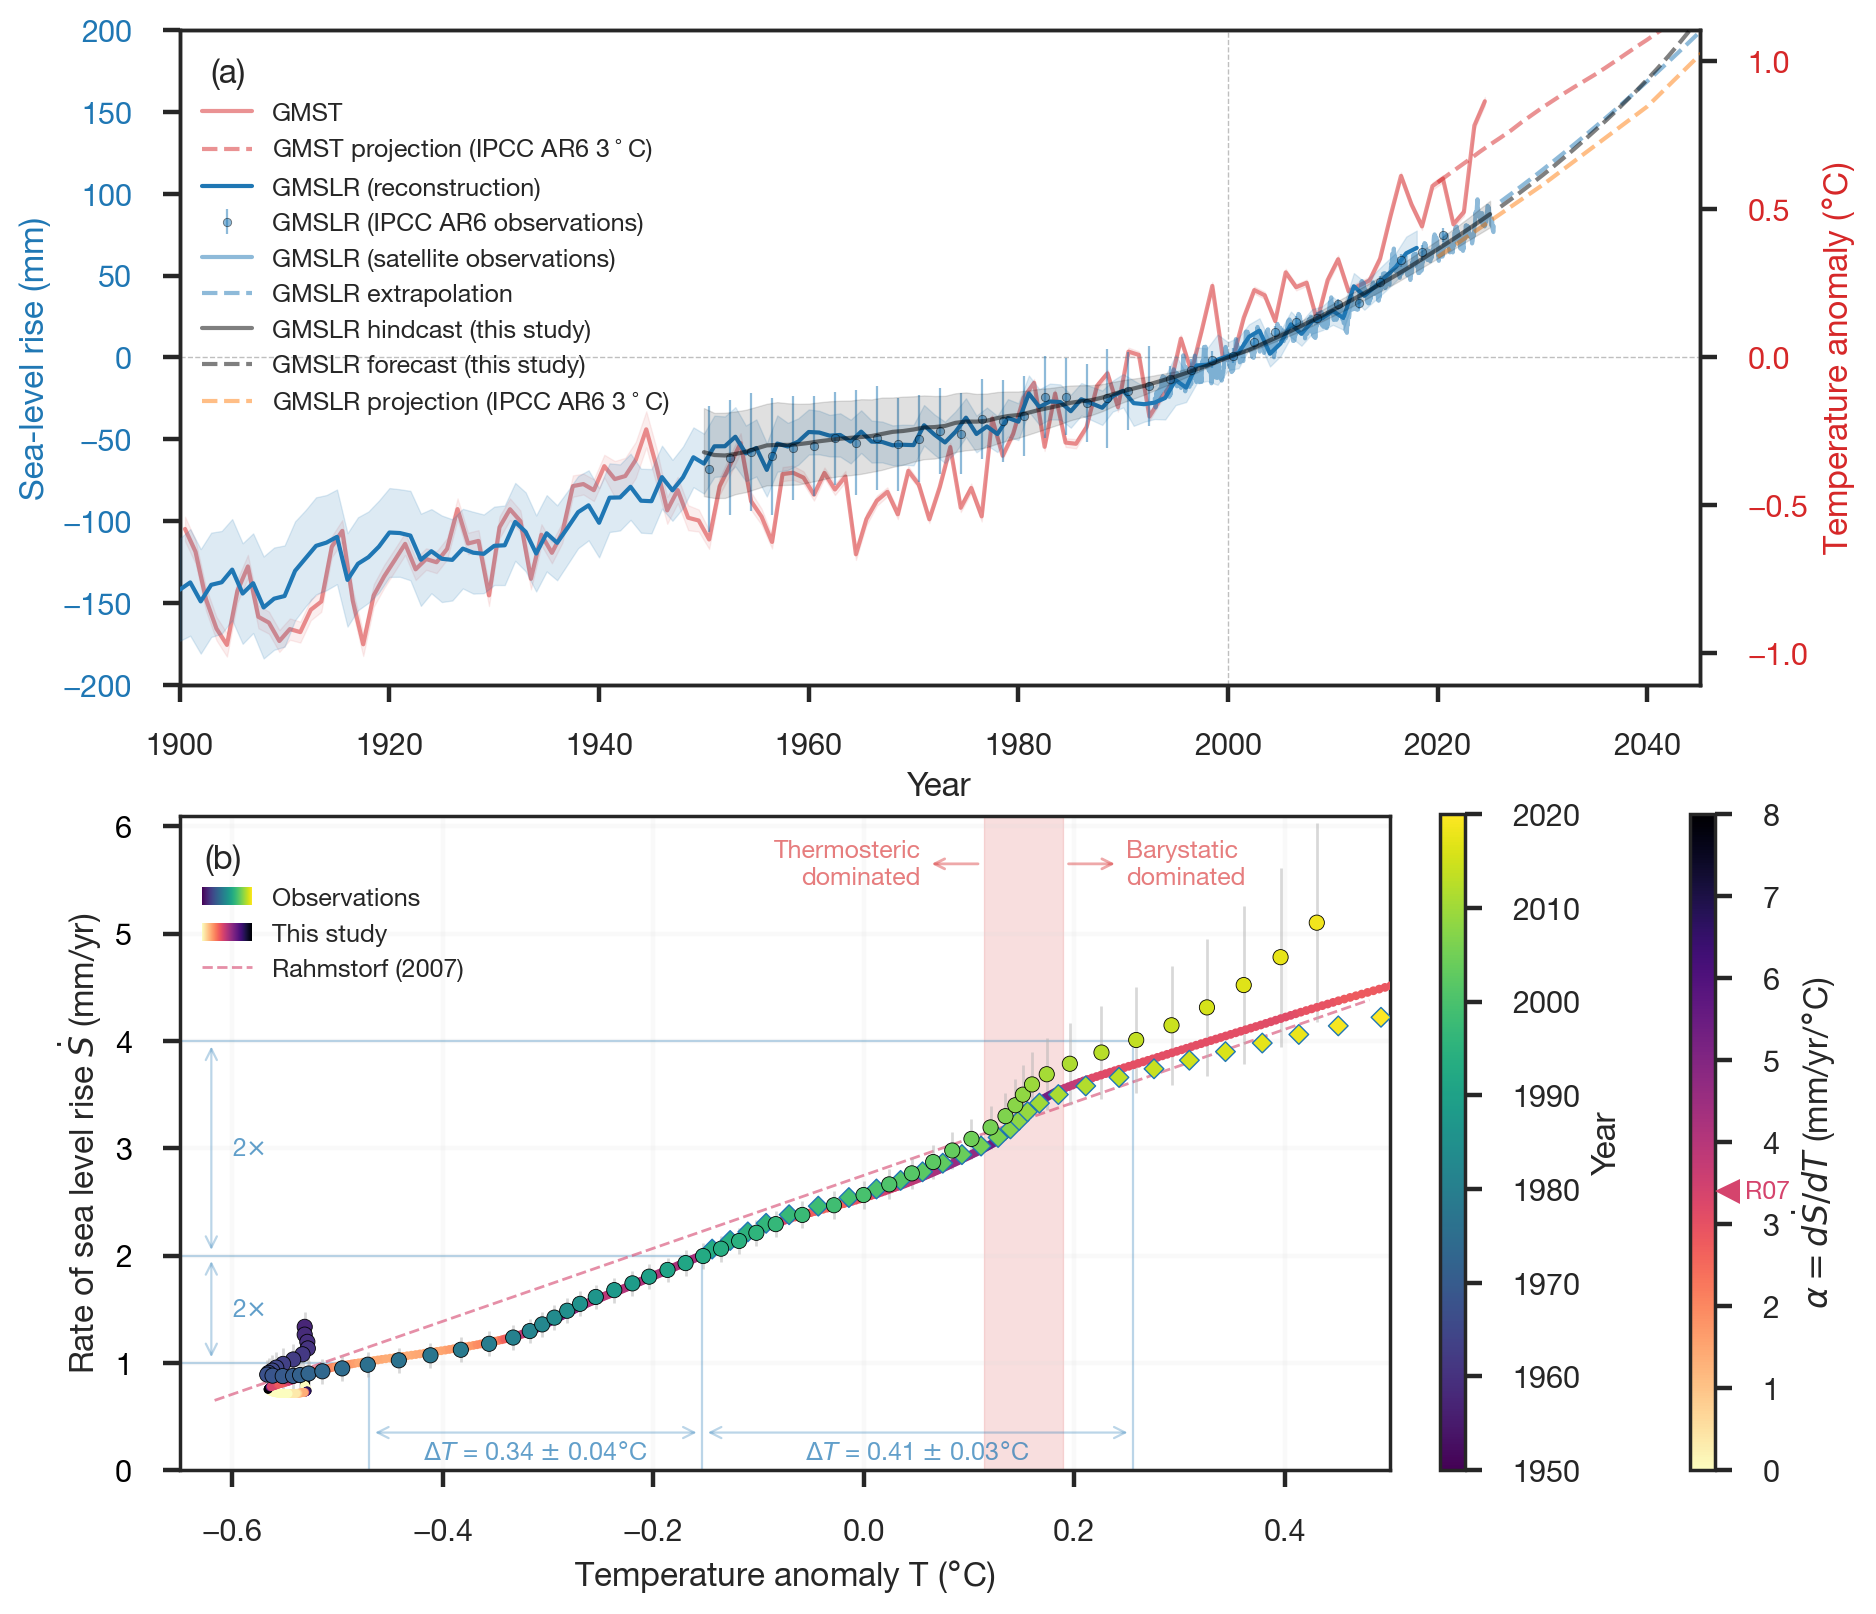
\includegraphics[width=\textwidth]{fig1v2_observations.png}
\caption{\textbf{Observed global mean sea-level rises with global mean surface temperature.}
\textbf{(a)} GMSLR from reconstructions and tide-gauge records (blue line \citealp{Frederikse2020}; blue circles \citealp{Fox-Kemper2021}) along with more recent NASA satellite altimetry (light blue; \citealp{Beckley2017}) show sea-levels rising with warming. Hindcast results of this study (grey line with 90\% CI shading) show good agreement back to 1950, the earliest year when GMSL reconstructions agree \citep{Fox-Kemper2021}. Different projection methods (dashed lines) show the divergence of IPCC AR6 projections and observed trends within a decade. GMST (red; \citealp{Rohde2020}) is referenced to the right hand axis.
\textbf{(b)} Rate of GMSLR ($\dot{S}=dGMSLR/dt$) versus GMST anomaly, $T$.  Observed values are shown in circles \citep{Frederikse2020} and diamonds \citep{Beckley2017}, colored by year, and the component model of this study is a line colored by instantaneous transient sensitivity $\alpha = d\dot{S}/dT$. The Rahmstorf (2007) semi-empirical model is shown in a color corresponding to its $\alpha$ value \citep{Rahmstorf2007}. The vertical red band indicates the shift in the primary contributor from ocean thermal expansion to changes in glacier ice and water storage (barystatic). The sinuous tail in the early observations is largely due to dam impoundment of water rather than a thermodynamic signal~\citep{Frederikse2020}. }
\label{fig:observations}
\end{figure}

Every centimeter of sea-level rise exposes roughly 1.6 million additional people to annual coastal flooding \citep{Kulp2019}, approximately 90\% of whom live in low- and middle-income countries \citep{Jongman2012}. Without additional adaptation, annual flood damages are projected to reach US\$14--18T (trillion) per year for 0.9--1.1~m of rise \citep{Jevrejeva2018}. Estimates of total adaptation costs per unit sea level rise are not available but a lower-bound, rough-order-of-magnitude estimate of US\$4T per meter of sea-level rise is reasonable based on a projected cost of US\$400B simply to raise dikes by 1 meter along only 3.4\% of coastlines \citep{Tiggeloven2020}. Developing countries currently receive US\$21B per year in total adaptation finance across all sectors, not just coastal \citep{UNEP2023}, raising questions about the feasibility of coastal adaptation at relevant scales.

%Rapidly resolving the uncertainties is essential because effective planning requires reliable sea-level forecasts be delivered before key decisions need to be made. Uncertainty in the rates of sea-level rise compounds uncertainty in inundation thresholds and paralyzes anticipatory spatial planning, routinely defaulting policy toward \emph{in situ} maladaptations that compound sunk costs and strand assets \citep{ODonnell2022}, or delaying action until forced by disaster \citep{Tubridy2021}. Unconstrained timelines encourage fragmented, market-based incrementalism that deploys public capital inefficiently \citep{SidersAjibadeCasagrande2021} and systemically transfers the financial burden of reactive retreat onto vulnerable municipalities and demographics \citep{SidersAjibade2021}. 

Current coastal adaptation planning relies heavily on projections from the IPCC Sixth Assessment Report (AR6), which estimates 0.4--0.7~m of rise by 2100 relative to the 1995--2014 baseline \citep{Fox-Kemper2021, Hirschfeld2023}. These projections depend on process-based ice sheet models forced with climate models and compared against one another in efforts such as ISMIP6 ***cite ISMIP6 papers***. Process-based ice sheet models represent the physics  

 %As a result, observed GMSL trends (0.66 m median at 2100, 0.41--0.91 m 90\% CI) are on track to exceed AR6 medium-confidence projections under all policy-relevant emission scenarios \citep{Hamlington2022, Hamlington2024}. AR6 documents this in a single figure but without comment: extrapolating the satellite-era rate and acceleration---which reflect the current warming trajectory that could lead to $3\ ^\circ$C (SSP2-4.5)---produces sea-level rise that matches or slightly exceeds the process-based projections under the very high emissions scenario (SSP5-8.5). %So while the data show that rates of sea level rise have doubled with approximately 0.4~$^\circ$C of warming (Fig.~\ref{fig:observations}b), IPCC models need roughly an order of magnitude more warming just to reproduce current observed rates of sea-level rise. 

In their current state, process-based models, diverge from historical records in hindcasting studies \citep{Aschwanden2021} and from satellite observations within a decade of initialization \citep{Fricker2025}. The reasons for the disagreements between observations and ice sheet models are manifold and described in greater detail in other publications ***. In essence, the disparities arise from known structural biases, including the absence of leading-order physical processes like iceberg calving \citep{Fricker2025} and an assumed ice viscosity that is less sensitive to changes in stress than observations indicate \citep{Millstein2022,GetraerMorlighem2025}, and initialization uncertainties. Decades of general forecasting research shows that models more complex than their calibration data can constrain generally produce worse predictions than simpler models \citep{Green2015}.

A forecasting system based on models representing diverse approaches and a hierarchy of complexity with robust testing against data can provide a foundation for reliable sea-level projections and guidance for the development of increasingly sophisticated, physics-based models that ***value for sea-level rise projections and to help guide the development of models that allow for deeper understanding of the salient physical processes. ***Finish paragraph on the value of different types of sea level forecast models***

The simplest are the data extrapolations, or ``naive'' forecasts. These approaches use observed GMSL rate and acceleration. The satellite altimetry record provides GMSLR measurements from 1993--2025 that show a constant acceleration of 0.08~mm\,yr$^{-2}$ (0.02--0.14~mm\,yr$^{-2}$) and rate 4.5~mm\,yr$^{-1}$ (3.5--5.5~mm\,yr$^{-1}$) in 2025 \citep{Hamlington2022, Hamlington2024}, already exceeding IPCC AR6 projections in 2025 (Fig. \ref{fig:ridge_projections}a). Extrapolating these values to 2100 yields 66~cm (41--91 cm) of 21st-century rise. Assuming the naive forecast has predictive skill over roughly half the calibration window, the extrapolation of the 32-year satellite record provides predictive skill over the next 15-20 years. Beyond that horizon, the naive forecast is less reliable but nevertheless establishes a scenario-independent, data-driven reference (Fig. \ref{fig:ridge_projections}a). 

The next class of data-driven forecasts are the semi-empirical models that fit the observed sensitivity of the rate of GMSLR to changes in GMST (Fig.~\ref{fig:observations}b). Under current warming trends, Rahmstorf (2007) \citep{Rahmstorf2007} predicts 0.67~m (0.63--0.71 m) of 21st-century rise, matching the naive forecast and the results of this study within error. Although physically motivated by the fit to observed sensitivities, semi-empirical models were assessed as \emph{low confidence} by IPCC AR5 because they do not resolve individual contributing processes and because extrapolation beyond the calibration period assumes a stationary temperature--sea-level relationship \citep{Church2013}. This reasoning is carried forward by AR6 but is violated by the decision to favor process-based models that omit key physical processes, are initialized to snapshots of non-stationary data, and were not tested against observed GMSL, the very quantity they claim to predict, prior to publication \citep{Fox-Kemper2021}. In short, the old adage holds that all models are wrong, and in the case of predicting future sea level rise, a framework leveraging a hierarchy of model complexity leverages the relative strengths of different approaches, providing clearer, more concrete connections with data and allowing for comparison across models that differ structurally. 

At the next level of complexity are the component-summation approach complements and is differentiated from previous studies \citep{Kopp2014,Mengel2016,Wong2017} by the models used for the individual components, the data used in the calibration, the approach to estimating uncertainties, and the anchoring of the projections in the near-term to the observed trends. ***Briefly describe existing models*** 


Here, we construct a data-driven framework that treats individual sea-level contributors with their own parsimonious physical models constrained by independent observational records. We name the framework the Sea-level Projections from Empirical Calibration of Thermodynamical, RedUced-physics Models (SPECTRUM). The individual components include ocean thermal expansion (thermosteric), Greenland Ice Sheet (GrIS) surface mass balance (SMB) and glacier discharge, West Antarctic Ice Sheet (WAIS) glacier discharge, East Antarctic Ice Sheet (EAIS) SMB, Antarctic Peninsula total ice loss, glaciers (land ice not in the ice sheets), and terrestrial water storage. Many of the component models are adopted from the literature. In these cases, the main contribution from this study being the data calibration and forecasting approaches. The exception is Greenland Ice Sheet dynamics, whose parsimonious model connecting glacier discharge and ocean temperature is unique to and developed in this study. 

As an overview on validation, we note that observed GMSLR and its sensitivity to observed global mean surface temperature (GMST) are withheld from the calibration of the components and serve as diagnostics for the composite model where the individual components are added. Unless otherwise noted, all sea-level values in the main text are global-mean 21st-century contributions referenced to the year 2000. Throughout, emission scenarios are labeled by their approximate median end-of-century global mean surface temperature rounded to the nearest integer: 2$\,^\circ$C (SSP1-2.6), 3$\,^\circ$C (SSP2-4.5), and 4$\,^\circ$C (SSP3-7.0).




\section{A data-driven, component-level projection framework}
%% ================================================================


***remove or move*** while extending to more recent data, initializing the forecasts by blending the calibrated sensitivities with extrapolated observational trends to ensure near-term alignment between the forecast and observed trends (Supplementary Materials), and developing a structured deep-uncertainty treatment of WAIS discharge. The sensitivities of glaciers, GrIS discharge, and Antarctic Peninsula to warming are calibrated with independent observational datasets spanning 24--71 years (Table~S1). Surface mass balance for GrIS and EAIS are adopted from published model sensitivities rather than data calibration because they lack sufficient data coverage for our approach \citep{Fettweis2020, Noel2021}. For completeness, we adopt the IPCC projection of terrestrial water storage due to a lack of suitable data to service a data-driven approach. Details of our models for EAIS and Antarctic Peninsula can be found in Supplementary Materials; we omit them from the main text because their contributions are small enough to be within the uncertainties of the primary contributors. 

%% ---- Figure 2: Model calibration, validation, and WAIS uncertainty ----
\begin{figure}[t]
\centering
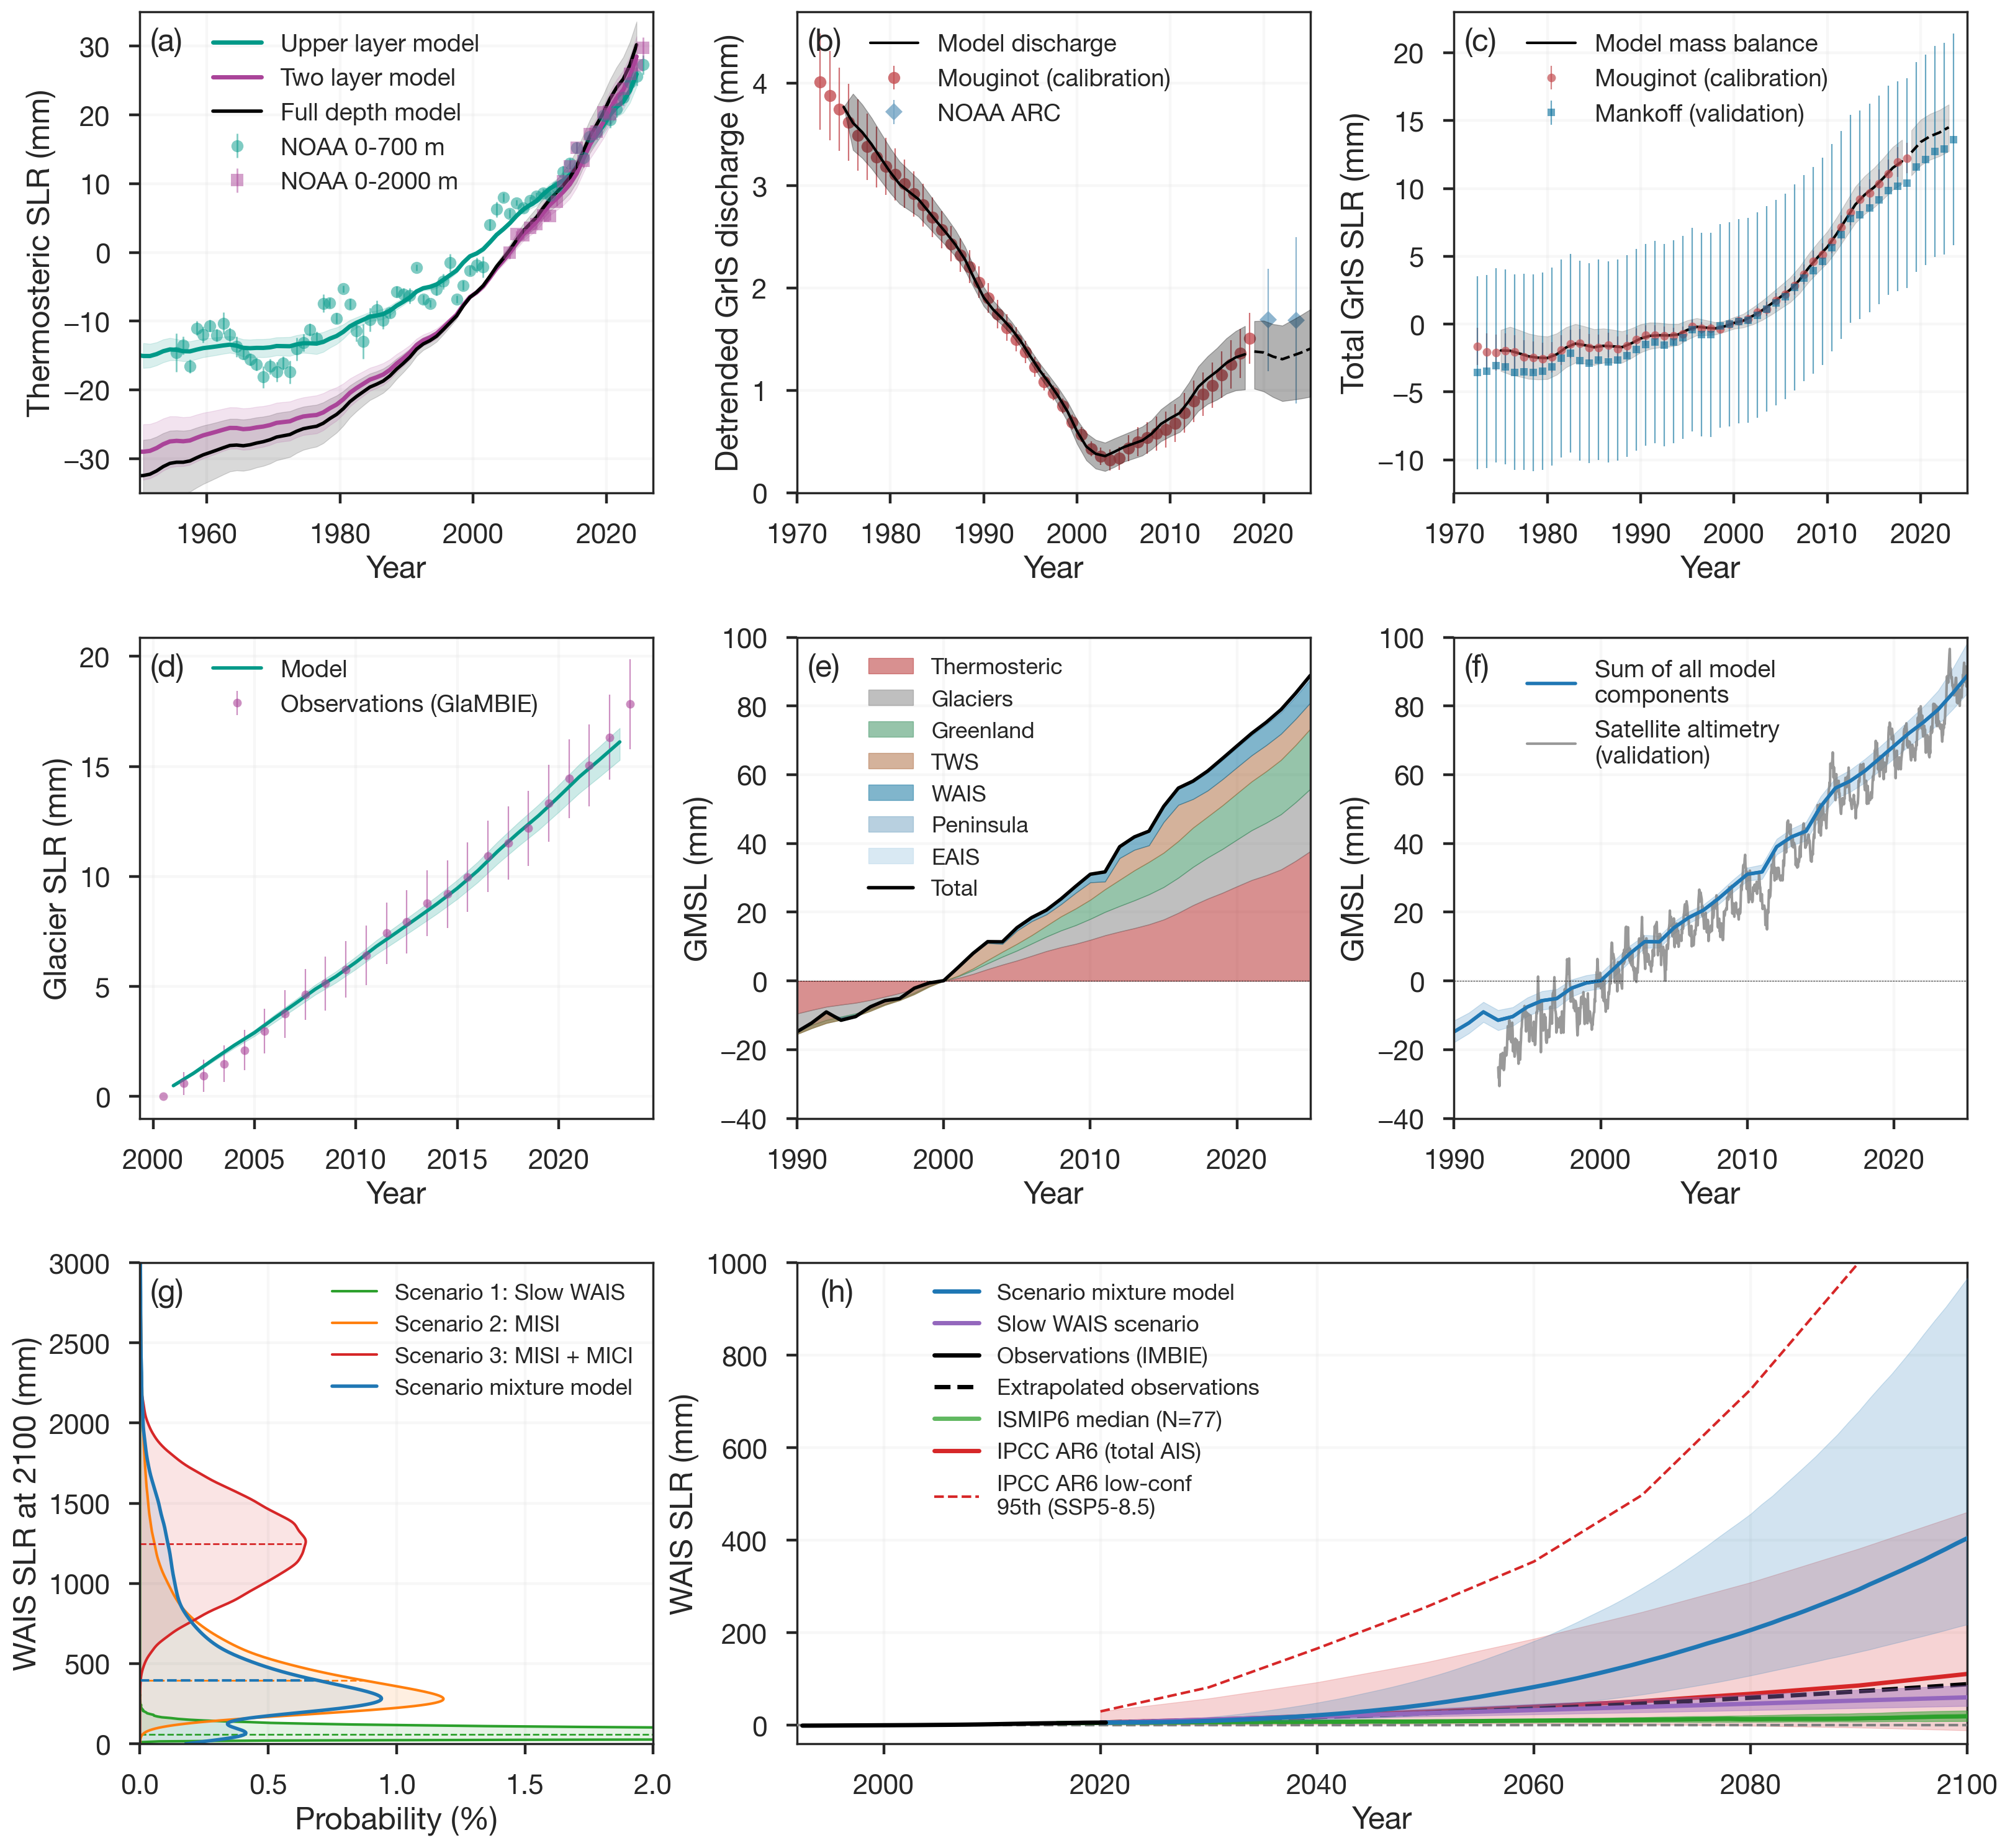
\includegraphics[width=\textwidth]{fig3_calibration_validation.png}
\caption{\textbf{Model calibration, validation, and WAIS uncertainty.}
\textbf{(a)} Our two-layer energy balance model fitted jointly to NOAA thermosteric values at different depth layers with the full depth model used in the forecasts (Supplementary Materials). 
\textbf{(b)} Greenland ice discharge modeled as a cumulative time-delay response to subsurface ocean warming with the calibration data from \citep{Mouginot2019} shown with filled circles and diamonds showing NOAA Arctic Report Card estimates \citep{Poinar2026}.
\textbf{(c)} Greenland total mass balance with validation data shown in blue squares with 90\% CI error bars \citep{Mankoff2021}.
\textbf{(d)} Global glacier model fitted to GlaMBIE consensus observations (2000--2023) using a linear temperature-driven model.
\textbf{(e, f)} Budget closure: temperature-forced component hindcast (stacked) compared with satellite altimetry data (cf. Fig. \ref{fig:observations}).
\textbf{(g)} WAIS scenario distributions at year 2100; dashed lines indicate medians. 
\textbf{(h)}WAIS projections from our full scenario mixture (blue) and slow WAIS scenario (purple) compared with  observations (black, \citealp{Otosaka2023}), the ISMIP6 ensemble (green; \citealp{Seroussi2020}), and IPCC AR6 projections (red). }
\label{fig:calibration}
\end{figure}

\subsection{Component models and calibration}

\subsubsection{Greenland Ice Sheet}

The Greenland Ice Sheet (GrIS) is the largest land-ice contributor and has lost mass every year since the 1990s \citep{Mouginot2019,Mankoff2021}. That loss is the imbalance between solid-ice discharge and surface mass balance (SMB), the difference between mass gained by snow accumulation and mass lost to melting. SPECTRUM treats the two separately, taking SMB from regional climate models *** and calibrating discharge against observations. 

GrIS discharge is sensitive to ocean temperature and surface melt runoff \citep{Straneo2013,Slater2020,Wood2021}. Warm, subsurface waters thin and undercut the calving fronts of marine-terminating glaciers, driving increased calving and net terminus retreat. This effect is amplified where surface runoff drives mixing and buoyant upwelling along the calving face \citep{Slater2022}. Surface melt also lubricates glacier beds, but that effect is generally short-lived and localized as the subglacial hydrological system evolves to accommodate changes in meltwater flux \citep{Schoof2010,Tedstone2013,Ultee2022}.
 
We calibrate SPECTRUM against total GrIS discharge, integrated across the 219 marine-terminating outlet glaciers resolved in the observational record \citep{Mouginot2019}. This integration is an intentional trade-off of spatial resolution for signal-to-noise. Given the strong influence of ocean-induced melting on discharge, we approximate the GrIS-wide discharge as
\begin{equation}
	D = \gamma\,T_{\mathrm{ocean}}(t - \delta) + r_0,
	\label{eq:greenland_rate}
\end{equation}
where $D$ is the GrIS discharge in sea-level equivalent units, $\gamma$ is an effective discharge sensitivity to ocean temperature, $\delta$ is the lag between distal ocean warming and ice sheet response, $r_0$ is the background discharge rate at the baseline ocean temperature, and $T_{\mathrm{ocean}}$ is the ocean temperature anomaly in the peripheral waters around Greenland relative to the 1995--2005 mean. Because $D$ is the gross discharge flux rather than an anomaly, it becomes a contribution to GMSLR only when combined with SMB, whose accumulation term offsets most of the background rate $r_0$. 

We calibrate the time-integrated form of Eq.~\ref{eq:greenland_rate} to get the
cumulative contribution of GrIS discharge to GMSLR,
\begin{equation}
\label{eq:greenland_dyn}
      \Delta H_{\mathrm{D}}(t) = \gamma \int_{t_0}^{t} T_{\mathrm{ocean}}(t' - \delta)\, dt' + r_0\,(t t_0),
\end{equation}
where $t_0$ is the start of the calibration record and $\gamma$ and $r_0$ are constant in time. Fitting the time-integrated (cumulative) record improves the signal-to-noise ratio, because the cumulative signal grows linearly in time while the annual errors accumulate only as its square root. It also directly constrains the total mass lost, the quantity of interest in this study.

\begin{figure}[ht]
\centering
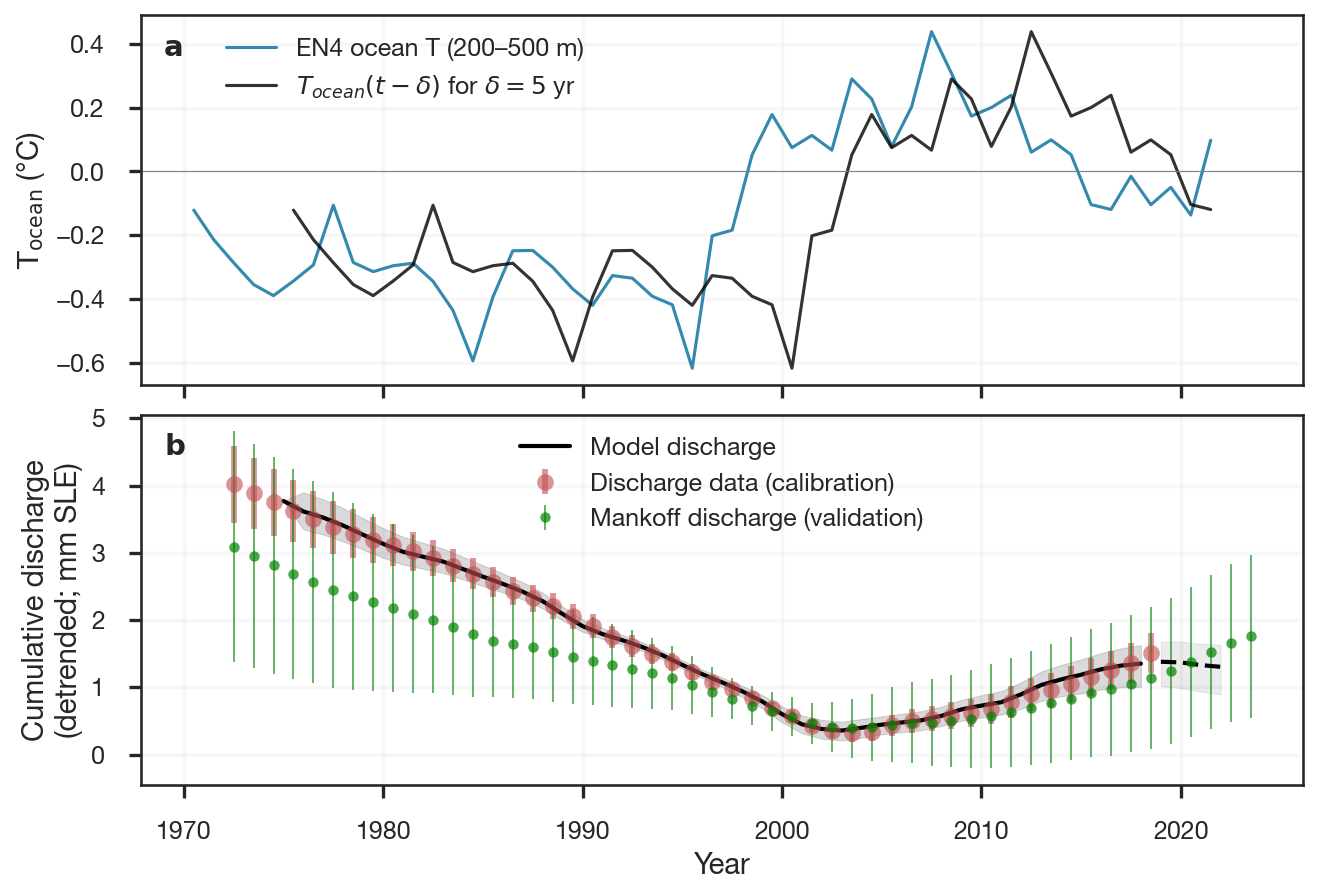
\includegraphics[width=\textwidth]{component_greenland_discharge_delay_fit.png}
\caption{\textbf{Greenland discharge delay model fit.} \textbf{(a)} EN4 subsurface ocean temperature (200--500\,m, annual) and the delayed signal $T_{\mathrm{ocean}}(t-\delta)$ with $\delta = 5$\,yr. \textbf{(b)} Detrended cumulative Greenland ice discharge showing model fit (black) with 90\% posterior CI, compared with the calibration \citep{Mouginot2019} and validation data \citep{Mankoff2021} in red and green, respectively. }
\label{fig:greenland_delay_fit}
\end{figure}

The calibration uses 47 years of glacier discharge data \citep{Mouginot2019} and ocean temperatures from EN4 (v4.2.2, g10 bias correction) \citep{Good2013}, averaged over 200--500\,m depth, the range most relevant to Greenland's tidewater grounding lines \citep{Slater2020}, in the seas surrounding Greenland south of
80$^\circ$N (58--80$^\circ$N, 75--5$^\circ$W), a limit set by the sparse subsurface sampling farther north (Fig. \ref{fig:greenland_delay_fit}). Because the data are resolved annually, the lag $\delta$ is in integer-year values. We therefore fit $(\gamma, r_0)$ by weighted least squares separately for a range of $\delta$ values, using the demeaned cumulative record. Each fit carries a penalty on the mismatch between the modeled discharge rate at the end of the record and the rate observed over the final decade, which keeps the calibration consistent with the present-day discharge rate. The posterior is then formed as a Gaussian mixture of the per-$\delta$ fits, with weights derived from the Bayesian Information Criterion. This procedure places 99.5\% of the weight on $\delta = 5$~yr (rate-space $R^2 = 0.794$) and gives posterior medians $\gamma = 0.365$~mm\,SLE\,yr$^{-1}\,^\circ$C$^{-1}$ (90\% CI, 0.312--0.419~mm\,SLE\,yr$^{-1}\,^\circ$C$^{-1}$) and $r_0 = 1.383$~mm\,SLE\,yr$^{-1}$ (90\% CI, 1.367--1.399~mm\,SLE\,yr$^{-1}$). The calibration target is a cumulative record, resulting in correlated, so we report parameter intervals from a covariance that accounts for that correlation and for the excess scatter of the residuals relative to the reported observational errors ($\chi^2/\mathrm{dof} = 1.8$), rather than from the least-squares covariance, which assumes independent errors. We validate the model against a discharge record spanning 1986--2023 that was withheld from calibration \citep{Mankoff2021}. This is a weak, but nonzero, validation because the \citet{Mouginot2019} and \citet{Mankoff2021} records are independently calculated from the same raw data. Our model falls within error of validation data, as does the total Greenland contribution to GMSLR (Fig. \ref{fig:calibration}c). The validation results suggest that our simple model, with two fitted parameters and a selected lag, captures the total contribution of GrIS discharge to GMSLR during the observational record and its sensitivity to ocean temperatures in Greenland's peripheral waters.

The fitted $\delta = 5$~yr is an effective lag for spatially averaged forcing and we therefore do not attempt to attribute it to a single process. It lies within the range of timescales spanned by the ocean-to-ice pathway, from exchange between the continental shelf and fjord interiors through the terminus response to undercutting and the inland transmission of retreat to the flux gates at which discharge is measured \citep{StraneoHeimbach2013,Wood2021,robel_response_2018}. Because $T_{\mathrm{ocean}}$ is averaged over Greenland's peripheral waters, $\delta$ also absorbs the time required for a warming anomaly to become representative of conditions at outlet glaciers distributed around the ice sheet; retreat began in southeast and west Greenland in the mid-1990s and reached the northwest a decade later \citep{StraneoHeimbach2013}. 

No published study reports a Greenland-wide sensitivity of discharge rate to ocean temperature, so we derive a simple dimensional scaling to contextualize the inferred value $\gamma = 0.365$~mm\,SLE\,yr$^{-1}$\,$^\circ$C$^{-1}$. For a single outlet glacier, the submarine melt rate scales approximately linearly with ocean thermal forcing, the ocean temperature above the in situ freezing point $T_f$. Because $T_f$ is set by the pressure and salinity at the calving face and is effectively constant over the observational record, a change in thermal forcing equals a change in ocean temperature, and the melt-rate perturbation for glacier $i$ is
\begin{equation}
	\Delta \dot{m}_i = \kappa_i\,\Delta T_{\mathrm{ocean}},
	\label{eq:melt_rate}
\end{equation}
where $\kappa$ is the melt sensitivity to thermal forcing averaged over the submerged calving face. Plume parameterizations calibrated against Greenland observations \citep{Xu2013, Rignot2016, Slater2022} give a maximum melt sensitivity near the grounding line of 90--260~m\,yr$^{-1}$\,$^\circ$C$^{-1}$, and the face-averaged rate is two to three times smaller \citep{Wood2021}. We therefore take $\kappa = 36$--$104$~m\,yr$^{-1}$\,$^\circ$C$^{-1}$, with a central value of 60~m\,yr$^{-1}$\,$^\circ$C$^{-1}$. Submarine melt thins and undercuts the terminus, triggering calving and grounding-line retreat, such that the total ice flux perturbation is a factor $\mu$ times the direct submarine melt flux. For Greenland's tidewater glaciers, observations and models suggest $\mu = 3$--$10$ \citep{Enderlin2013, Wood2021}. The flux perturbation from a single glacier with submerged calving-front area $A_f$ is then
\begin{equation}
	\Delta \dot{Q}_i = \mu_i\,\rho_{ice}\,A_{f,i}\,\kappa_i\,\Delta T_{\mathrm{ocean}},
	\label{eq:single_glacier_flux}
\end{equation}
where $\rho_{ice} = 900$~kg\,m$^{-3}$ is the mass density of ice. Summing over Greenland's $N = 219$ marine-terminating outlets \citep{Mouginot2019} we have
\begin{equation}
	\gamma_{\mathrm{scale}} = \frac{1}{A_{\mathrm{ocean}}\,\rho_{fw}\,\Delta T_{\mathrm{ocean}}}\sum_{i=1}^{N} \Delta\dot{Q}_i ,
	\label{eq:gamma_aggregate}
\end{equation}
where $A_{\mathrm{ocean}} = 3.625 \times 10^{14}$~m$^2$ is the ocean area and $\rho_{fw} = 1000$~kg\,m$^{-3}$ is the density of fresh water, which converts added ice mass to sea-level equivalent under the convention 1~mm\,SLE~$= 362.5$~Gt used throughout this study. Submerged calving-front areas of 0.9--2.7~km$^2$ are reported for five West Greenland outlets \citep{Rignot2016}. Evaluating Eq.~\ref{eq:gamma_aggregate} across the full parameter ranges gives
\begin{equation}
	\gamma_{\mathrm{scale}} = 0.05\text{--}1.5~\mathrm{mm\,SLE\,yr}^{-1}\,{}^\circ\mathrm{C}^{-1},
	\label{eq:gamma_estimate}
\end{equation}
which contains our calibrated $\gamma = 0.365$~mm\,SLE\,yr$^{-1}$\,$^\circ$C$^{-1}$. We report Eq.~\ref{eq:gamma_estimate} as an order-of-magnitude check only. The range spans a factor of 30 because it is the product of four quantities that are not measured in aggregate, and the factorization $\sum_i \mu_i A_{f,i} \kappa_i \approx N\,\bar{\mu}\,\bar{A}_f\,\bar{\kappa}$ assumes these are uncorrelated across outlets, whereas the deepest and widest fronts occupy the warmest fjords. Finally, the calibrated $\gamma$ is an effective sensitivity that absorbs the covarying atmospheric pathway because increased subglacial runoff amplifies plume-driven melting alongside ocean warming. 



\subsubsection{Thermosteric}

The thermosteric component is currently the largest single contributor to observed sea-level rise. We model it with a two-layer thermal-response model with the deep-layer structure of \citet{Geoffroy2013}, fitted jointly to the NOAA objectively analyzed thermosteric sea level derived from \emph{in situ} profiles at 0--700\,m (1955--2025) and 0--2000\,m (2005--2025) \citep{Levitus2012} (Fig. ***). The model equations are
\begin{align}
\frac{dS_u}{dt} &= \frac{T(t) - S_u}{\tau_u} \\
\frac{dS_d}{dt} &= \frac{S_u - S_d}{\tau_d} \\
H_{\mathrm{upper}}(t) &= a\,S_u^2 + b_u\,S_u + c\,(t - t_0), \label{eq:thermo_upper} \\
H_{\mathrm{total}}(t) &= H_{\mathrm{upper}}(t) + b_d\,S_d, \label{eq:thermo_total} \\
H_{\mathrm{full}}(t) &= H_{\mathrm{total}}(t) + \dot{H}_{>2000}\,(t - t_{\mathrm{ref}}), \label{eq:thermo_full}
\end{align}
where $S_u$ and $S_d$ are upper- and deep-ocean thermal state variables driven by GMST $T(t)$, $\tau_u$ is the upper-ocean relaxation time, $t_0 = 1850.5$ is the start of the GMST record, and $\tau_d = 150$\,yr is the deep-ocean relaxation time, fixed at the CMIP5 multi-model mean deep-ocean adjustment time $C_0/\zeta = 151$\,yr \citep[][Table 4]{Geoffroy2013}, where $C_0$ is the deep-ocean heat capacity and $\zeta$ the interlayer heat-exchange coefficient. We fix $\tau_d$ rather than sampling it because the 21-year 0--2000\,m record is too short to constrain centennial-timescale relaxation. Each record and its corresponding model prediction are demeaned before comparison, so the fit carries no intercept and $t_0$ sets only a constant offset. Equations \ref{eq:thermo_upper} and \ref{eq:thermo_total} are the quantities fitted to the 0--700\,m and 0--2000\,m records. The forecasts use $H_{\mathrm{full}}$, which adds the ocean below 2000\,m as a constant rate $\dot{H}_{>2000} = 0.07 \pm 0.04$\,mm\,yr$^{-1}$ \citep{Purkey2010} referenced to $t_{\mathrm{ref}} = 2000$; this layer is not observed at annual resolution, so it is adopted rather than calibrated. 

The six free parameters ($a$, $b_u$, $b_d$, $c$, $\log\tau_u$, $\log\sigma_{\mathrm{extra}}$) are sampled via MCMC (emcee; 48 walkers, 4000 burn-in + 12000 production steps). The posterior median and 90\% credible intervals are: $a = 19.2$~[9.5, 29.2]~mm\,$^\circ$C$^{-2}$, $b_u = 50.0$~[40.0, 70.7]~mm\,$^\circ$C$^{-1}$, $b_d = 67.2$~[36.1, 100.9]~mm\,$^\circ$C$^{-1}$, $c = 0.023$~[$-0.107$, 0.137]~mm\,yr$^{-1}$, $\tau_u = 11.0$~[5.9, 22.9]~yr, and $\sigma_{\mathrm{extra}} = 2.0$~[1.7, 2.3]~mm. The calibrated model reproduces both records with RMS residuals of 2.3~mm for depths 0--700\,m and 1.3~mm for 0--2000\,m, against 42 and 30 mm of observed rise over the respective records.

\begin{figure}[ht]
\centering
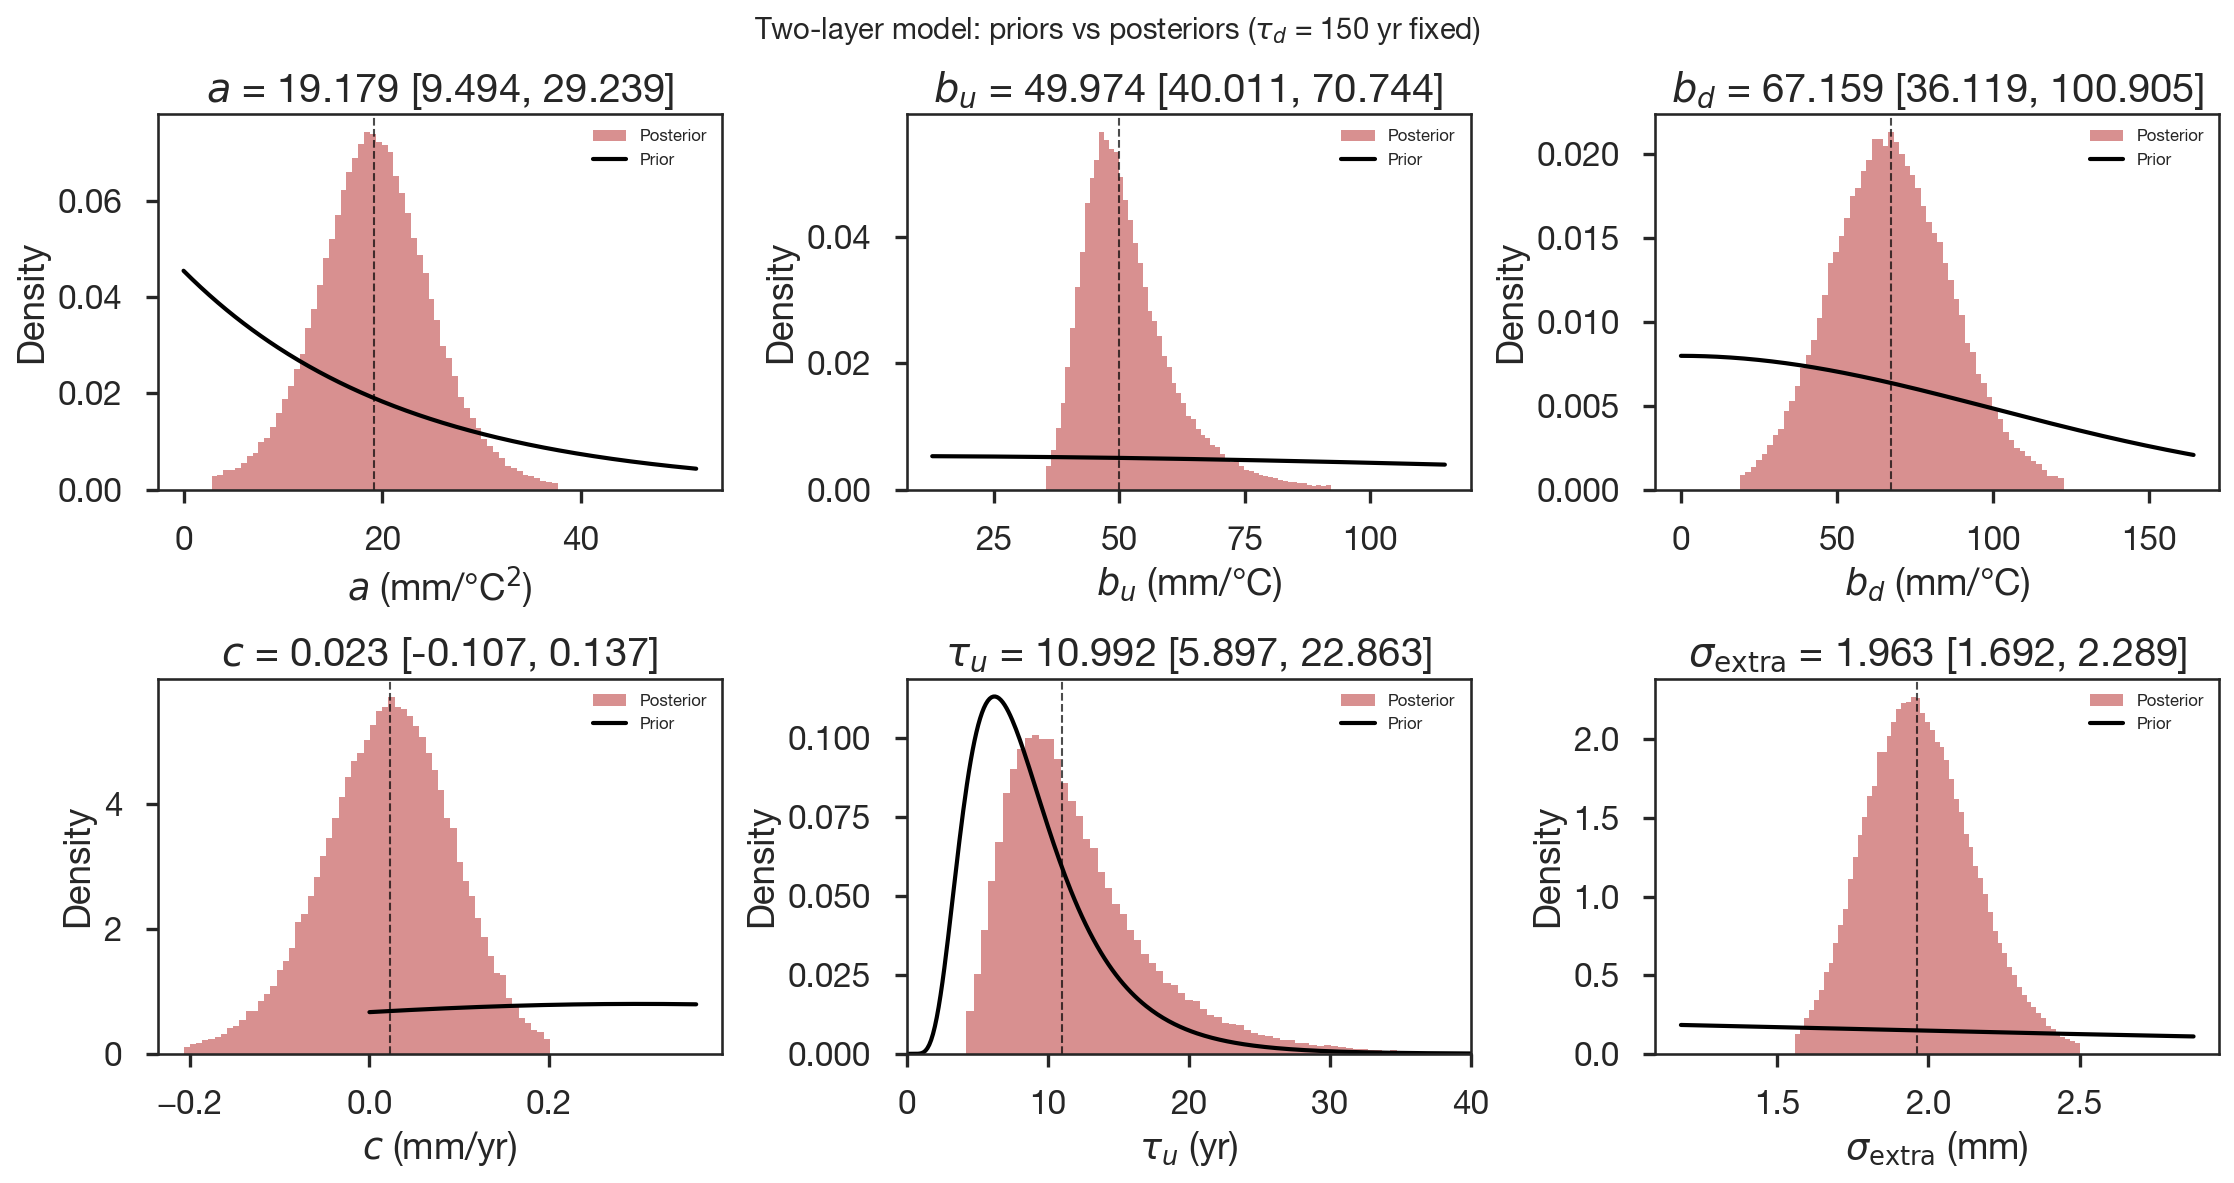
\includegraphics[width=\textwidth]{component_ocean_priors_posteriors.png}
\caption{\textbf{Two-layer thermosteric model: priors and posteriors.} Prior distributions (black curves) and posterior histograms (red) for the six parameters of the two-layer energy balance model fitted jointly to NOAA 0--700\,m and 0--2000\,m thermosteric sea level. Dashed vertical lines indicate the posterior median; panel titles report the median and 90\% credible interval. The deep-ocean relaxation time $\tau_d = 150$\,yr is fixed. For all parameters the posteriors are substantially narrower than and displaced from the priors, indicating that the observations---not the prior assumptions---are driving the inference. The one exception is $b_d$, whose posterior is wider than the others, reflecting the shorter 0--2000\,m record (21 years vs 71 years for 0--700\,m).}
\label{fig:ocean_priors_posteriors}
\end{figure}

%Because $a$ and $b_u$ multiply functions of $S_u$, which itself depends on $\tau_u$, a potential concern is parameter degeneracy such that changing $\tau_u$ rescales $S_u$, which could in principle be compensated by rescaling $a$ and $b_u$. Under full degeneracy, $b_u \propto \tau_u$ and $a \propto \tau_u^2$. The posterior does not exhibit this: $\tau_u$ varies by a factor of 3.9 across the 90\% CI, while $b_u$ varies by only a factor of 1.8 (not 3.9) and $a$ by a factor of 3.1 (not 15). This partial independence arises from four sources: (1)~the joint fit to two depth ranges with different time spans, where the deep-ocean response $b_d\,S_d$ provides an independent constraint on $\tau_u$ through the $S_u \to S_d$ coupling; (2)~the quadratic term $a\,S_u^2$, whose shape (curvature) changes with $\tau_u$ and cannot be compensated by a simple rescaling of $a$; (3)~the interannual and decadal variability in GMST, which constrains the phase lag of $S_u$ relative to $T(t)$ independently of amplitude; and (4)~the trend term $c\,(t - t_0)$, which is entirely $\tau_u$-independent. Pairwise posterior correlations are moderate ($|r| < 0.7$ for all parameter pairs), and no bimodal structure is evident in the posterior. Corner plots are provided in the analysis notebook.

The ODE system is solved via an exponential integrator (piecewise-constant midpoint forcing, analytical decay) with initial conditions $S_u(0) = S_d(0) = T(0)$ (equilibrium assumption). 


***To generate projections, we drive the fitted model with IPCC AR6 SSP temperature trajectories, propagating posterior parameter uncertainty, SSP temperature trajectory uncertainty, and below-2000\,m rate uncertainty ($0.07 \pm 0.04$\,mm\,yr$^{-1}$) via 2,000 Monte Carlo samples. ***Forecasts are generated by driving the calibrated two-layer model with IPCC AR6 temperature trajectories, propagating posterior parameter uncertainty via Monte Carlo sampling (Supplementary Material).

\begin{figure}[ht]
\centering
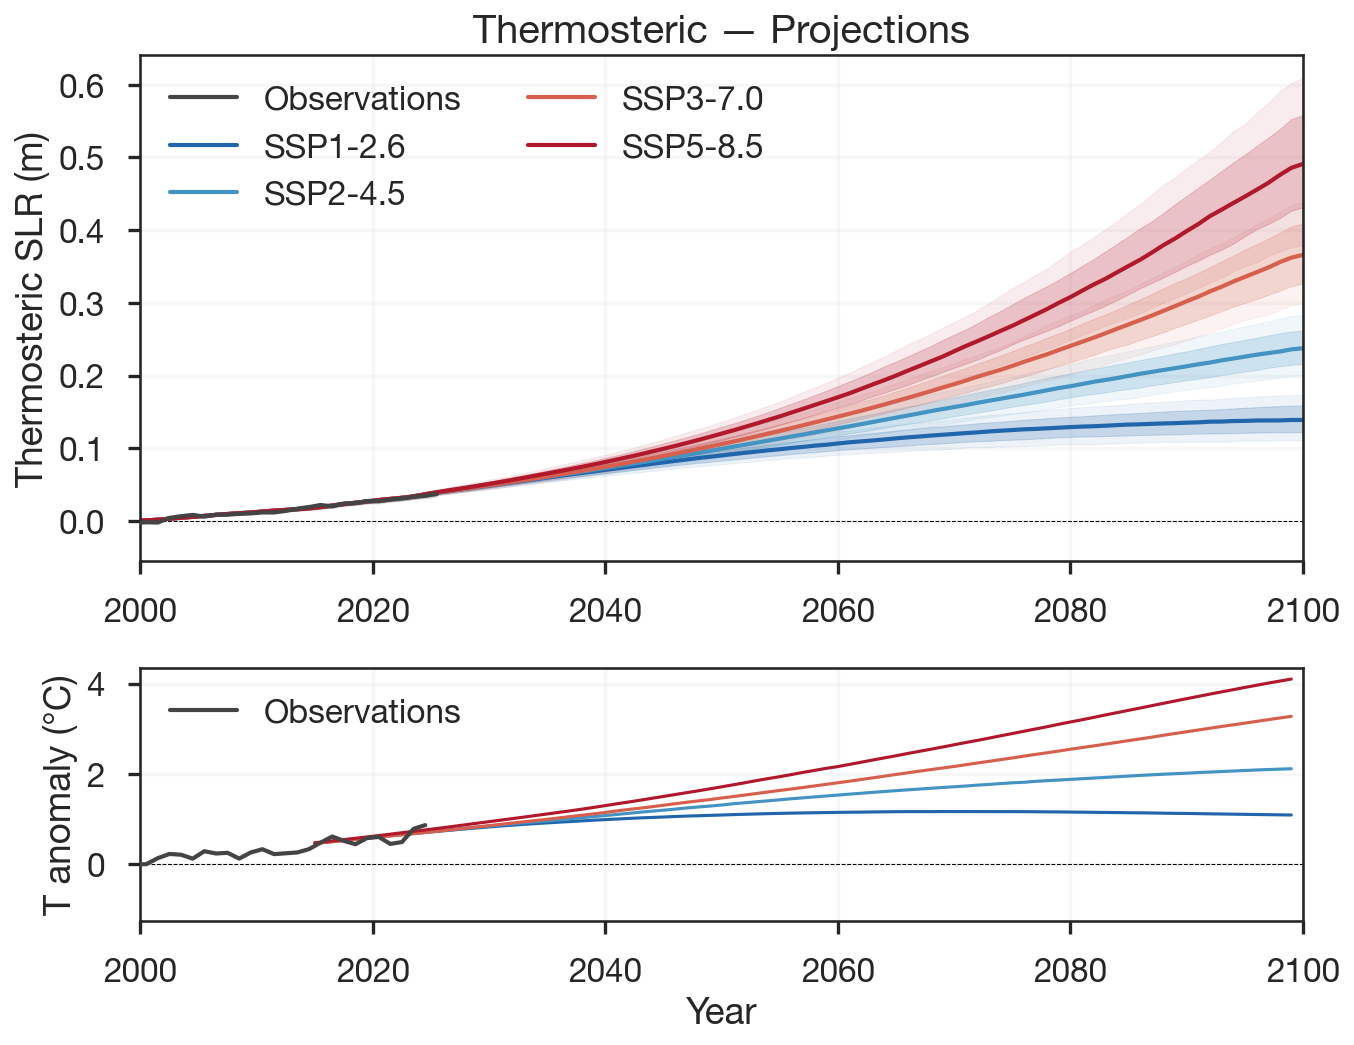
\includegraphics[width=0.85\textwidth]{component_ocean_twopanel.png}
\caption{\textbf{Thermosteric sea-level projections.} Upper panel: median and 66\%/90\% credible intervals for the two-layer model under four SSP scenarios, with full-depth observations (black). Lower panel: GMST forcing trajectories (relative to year 2000) with Berkeley Earth observations.}
\label{fig:ocean_twopanel}
\end{figure}




\subsubsection{Glaciers}

Mountain glacier mass loss is modeled as a rate--temperature relation calibrated against the GlaMBIE global consensus \citep[2000--2023;][]{GlaMBIE2025} and GMST. The data only support a linear sensitivity (Supplementary Material), which we find to be $b_{\mathrm{gl}} = 0.66$~mm\,yr$^{-1}$\,$^\circ$C$^{-1}$ (Fig. \ref{fig:calibration}d). This is approximately five times the value embedded in IPCC AR6 median projections ($\sim$0.13~mm\,yr$^{-1}$\,$^\circ$C$^{-1}$) and 1.3--1.7$\times$ the effective sensitivity of the PyGEM process model \citep{Rounce2023}, but provides excellent fit with global data compilations.

\subsubsection{Antarctic Peninsula} 

\subsubsection{East Antarctica}

\subsection{Forecasting approach}


To project GrIS discharge model forward in time, we calibrate a transfer function between the Greenland regional surface temperature anomaly and the ocean temperature and then apply a normal distribution of Arctic amplification factors to calculate the Greenland regional surface temperature form projected GMST under different emission scenarios (Supplemental Material). For SMB, we adopt published linear and quadratic sensitivities of SMB to GMST from RCM intercomparisons \citep{Fettweis2020, Noel2021}, using the spread across RCMs as structural uncertainty \citep{Glaude2024} 


\subsection{Component model validation}

For the hindcast, we use SMB reanalysis data \citep{Mouginot2019, Noel2018} directly.  

As a validation step, we compare the sum of the independently calibrated components to observations of GMSL from satellite altimetry (Fig.~\ref{fig:calibration}e,f). Validation is possible because each component is calibrated against its own observational record. Total GMSL is withheld from calibration. The component sum closes 93--101\% of the observed GMSLR rate over three epochs (1993--2025, 2000--2025, 2010--2025), with a variance-weighted attribution assigning the residual mainly to terrestrial water storage (45--56\%) and thermosteric (21--27\%) components, both within their stated uncertainties (Supplementary Material). The transient sensitivity of our component model, which defines the change in GMSLR rate with warming, closely agrees with observations and the Rahmstorf (2007) \citep{Rahmstorf2007} semi-empirical results (Fig. \ref{fig:observations}b).  



\subsection{West Antarctic Ice Sheet.} WAIS is the largest source of uncertainty in sea-level projections (Figs. \ref{fig:calibration}g,h). The ice sheet contains $\sim$3.3~m of sea level equivalent and rests on land that is below sea level and deepens inland, making it susceptible to internal feedbacks commonly called the marine ice sheet instability (MISI;~\citealp{Joughin2014}). The delivery of warm, deep seawater is the primary climate driver of mass loss \citep{Fricker2025}. Ocean thermal forcing sufficient to drive retreat is likely committed throughout the 21st century regardless of emissions pathway \citep{Naughten2023,Rosier2025} and may be driven as much by ocean processes local to the ice sheet as those further afield \citep{Moorman2023}. Based on these lines of evidence, we make our WAIS projections independent of the warming trajectory, meaning the range of 21st-century outcomes is controlled by ice dynamics that, to leading order, are insensitive to emissions over our forecasting horizon. 

No physical process models have been proven to reproduce observations \citep{Aschwanden2021} and we find insufficient data coverage and duration to support a data-driven forecast like those described above. To provide a representative range of uncertainties, we construct a scenario-mixture framework grounded in the scientific literature (Fig.~\ref{fig:calibration}g,h; Supplementary Material). Scenario 1: `slow WAIS' where rates of discharge continue to increase within the range of observed values and with linear relationship between SLR contributions and ocean temperatures. This scenario admits 25--85 mm GMSLR contribution by 2100. Based on the changes in WAIS discharge over the past decades and the position by the IPCC AR6, we take this scenario to be unlikely, and assign it a 10\% probability. Scenario 2 represents the role of MISI-driven acceleration and grounding-line retreat, yielding a GMSL contribution of 0.15--1 m by 2100. The lower value is anchored to transient-calibrated ice sheet model projections \citep{Goldberg2026} and the observed 33 km grounding-line retreat at Pine Island Glacier since 1992 \citep{Rignot2026} while the upper bound is set by structured expert judgment \citep{Bamber2019}. We assign Scenario 2 an 80\% probability. Scenario 3 represents MISI combined with the potential for cascading structural failure of ice cliffs, known as the marine ice cliff instability (MICI), with the range defined by the IPCC AR6 low-confidence 83rd (0.6 m) and 95th (1.3 m) percentile ranges. We assign a 10\% probability to this scenario, consistent with IPCC AR6 `deep uncertainty' framing. Within each scenario, the 2100 endpoint is drawn from a skew-normal distribution in log-space with physically motivated asymmetry \citep{Robel2019}. A multiplicative rheology correction ($R$ with median $R = 1.3$) is applied to all scenarios, reflecting the underestimation of ice loss when models assume the ice-viscosity stress exponent $n = 3$ rather than the observationally constrained value $n = 4.1\pm0.4$ \citep{Millstein2022,GetraerMorlighem2025,Martin2026}. The resulting mixture has a median 21st century sea-level rise of 0.41 m with a 0.07 to 1.56 m 90\% CI at 2100. We refer to this mixed model as `fast WAIS' because it allows for, but does not force, rapid ice mass loss (Scenarios 2 and 3). Sensitivity tests of the scenario weights show the chosen weights do not qualitatively impact the findings of this study (Supplementary Materials).

%% ================================================================
\section{Results}

We drive the calibrated model with the IPCC AR6 warming trajectories of 2 $^\circ$C (SSP1-2.6) through 4 $^\circ$C (SSP3-7.0), the pathways most consistent with current policies and stated pledges (Fig. \ref{fig:ridge_projections}). To ensure our sea-level trajectories are faithful to the observed trends in the first decade of the forecasting window, we smoothly blend extrapolations of observed trends for the next 10 years with the first 10 years of the forecasts so that the first year (2026) of our forecast is almost exclusively the extrapolated GMSLR rates from satellite observation, the forecast in 2031 has an even weighting between our component model and the naive forecast, and by 2036 the forecast is taken entirely from the calibrated components forced by different emission scenarios and warming trajectories.

For the 2$\,^\circ$C target, our forecast shows a median of 0.79 m of sea-level rise [0.46--1.89 m] relative to year 2000, which is 72\% above the IPCC AR6 medium-confidence estimate of 0.46 m. Under 3 $^\circ$C warming, approximately the current trajectory, the median is 0.96 m [0.62--2.07 m], 66\% above IPCC's 0.58 m. For the 4 $^\circ$C trajectory, the median reaches 1.16 m [0.82--2.26 m]. For reference, the 5 $^\circ$C warming trajectory (SSP5-8.5) yields a median of 1.35 m [0.99--2.45 m]. 

%% ---- Figure 3: Ridge + exceedance two-panel ----
\begin{figure}[t]
\centering
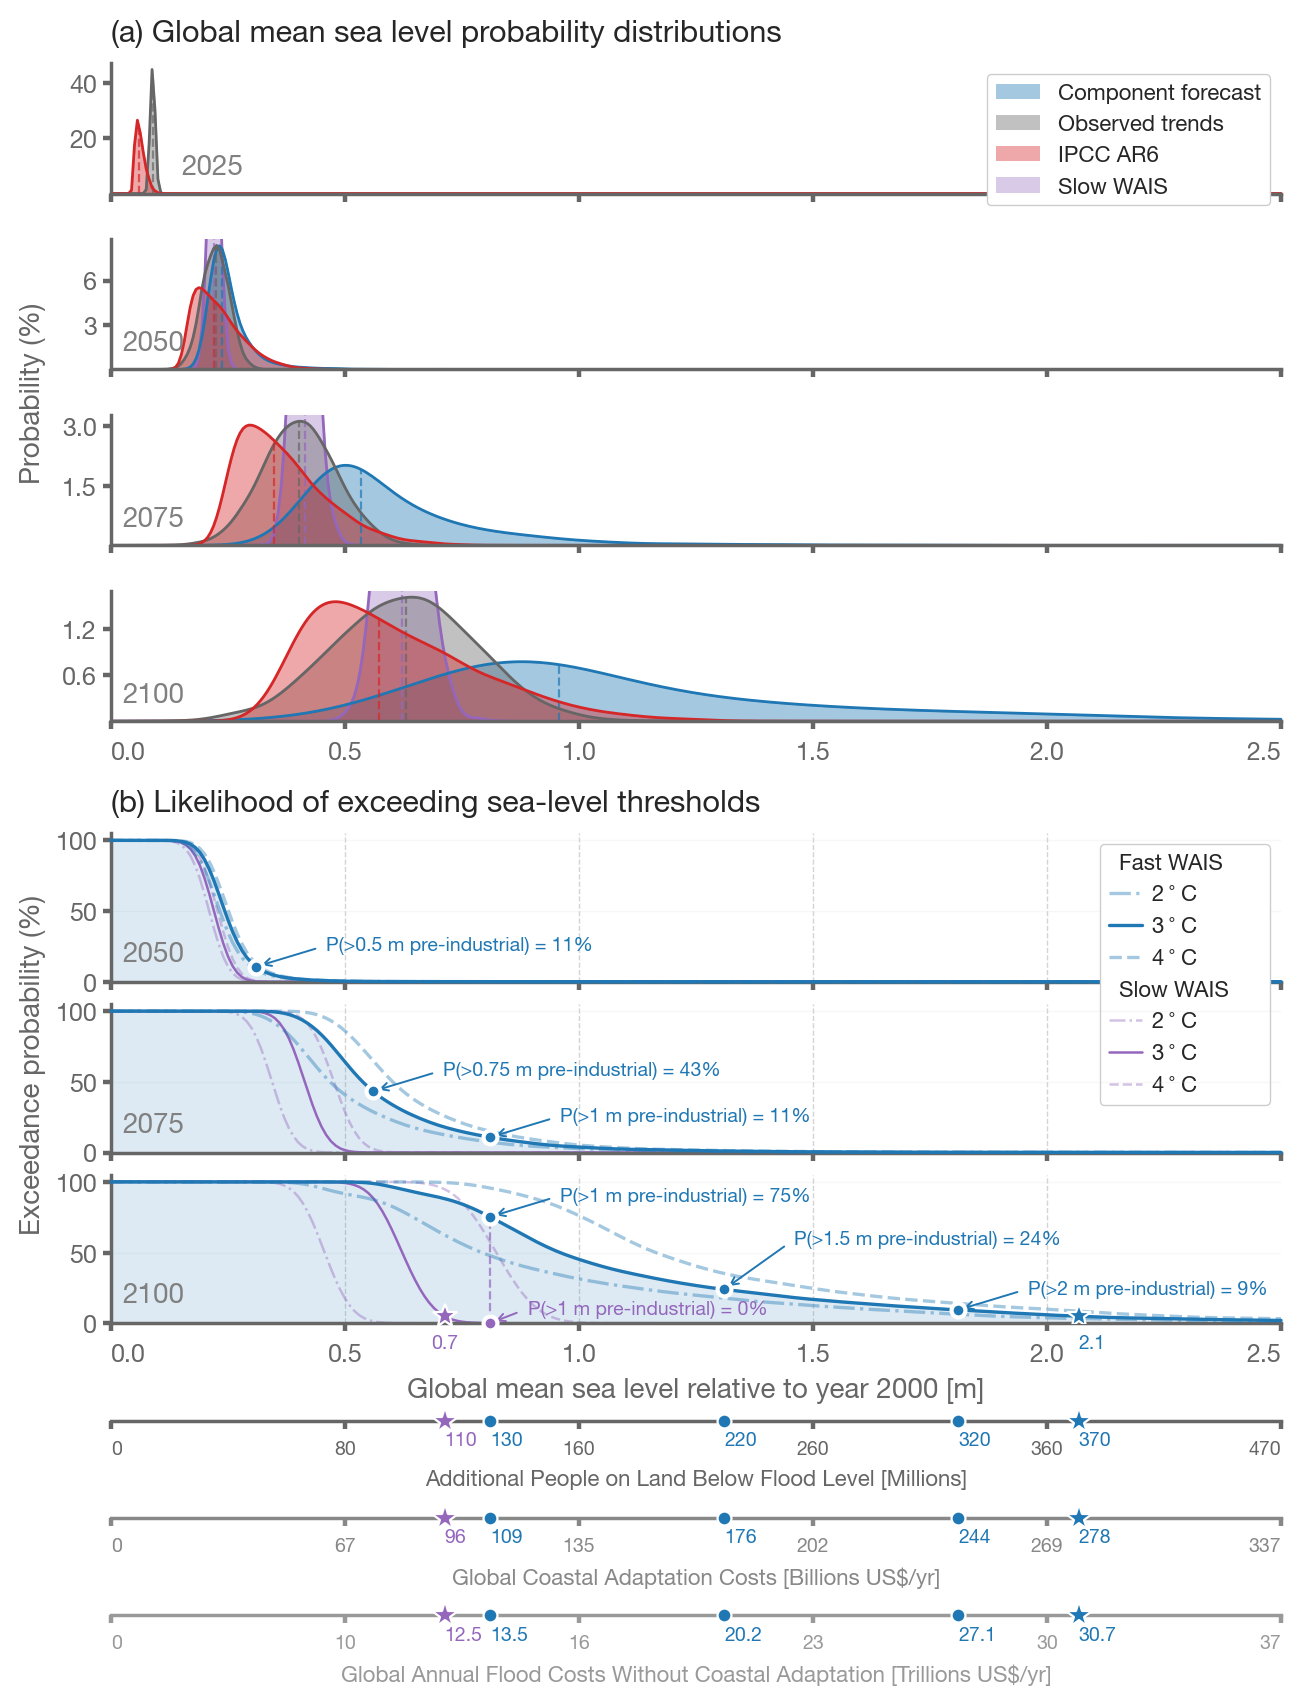
\includegraphics[width=0.85\textwidth]{fig2v2_ridge_exceedance.png}
\caption{\textbf{Global mean sea-level probabilities.}
(a) Probability distributions for different forecasting approaches and the IPCC projections. The `slow WAIS' scenario (purple, clipped for clarity) assumes sustained mass loss at approximately modern rates (Scenario 1). Vertical dashed lines indicate the respective medians. 
(b) Probability of exceeding a given sea-level threshold for different warming trajectories including the WAIS scenario mixture model that allows for fast mass loss (blue) and the slow WAIS scenario (purple). Lower axes show estimates of the corresponding number of people currently living on land that will be below flood level \citep{Kulp2019} and financial costs \citep{Tiggeloven2020,Jevrejeva2018} (Supplementary Material). Stars indicate the 5\% exceedance probability.}
\label{fig:ridge_projections}
\end{figure}

Relative to pre-industrial GMSL (adding $\sim$0.19 m of observed rise through 2000), these forecasts correspond to medians of 0.98--1.35 m of global mean sea level rise across the 2-4 $^\circ$C policy-relevant pathways. The probability of exceeding 1 m relative to pre-industrial by 2100 is 47\% under 2 $^\circ$C warming, 76\% under 3 $^\circ$C, and 96\% under 4 $^\circ$C warming trajectory. The probability of exceeding 2 m relative to pre-industrial by 2100 is approximately 10\%, with a minimum of 6\% if warming is held below 2 $^\circ$C. Under the condition that WAIS loses ice slowly, the probability of exceeding 1 m of sea level rise relative to pre-industrial levels effectively drops to zero for less than 3 $^\circ$C of warming, implying lower flood risks for tens of millions of people and reduced costs of adaptation and damages of order trillions of US dollars (Fig. \ref{fig:ridge_projections}b). As validation, our component forecast for 3 $^\circ$C of warming closely agreement with extrapolations of observed GMSLR trends, as should be expected if the warming trend remains similar to the current trend and WAIS, which has contributed only $\sim$4\% to GMSLR to date, continues to lose mass at its current rate. 

Across the range of possible WAIS mass loss and emission scenarios, our forecasts suggest that WAIS is likely to become the dominant source of sea-level rise before the end of the century (Fig. \ref{fig:components_voi}a). It is uncertain when that will happen and depends on how quickly emissions decrease. The stack of mean values shows the relative contributions of the primary sea-level contributors, showing that the thermosteric component likely will remain the single largest contributor in the 21st century unless WAIS mass losses over take it. Greenland and mountain glaciers will continue to lose mass and contribute to sea level rise throughout the 21st century. 

The distribution of the uncertainties shows a dramatic separation between the predictable and, currently, unpredictable components (Fig. \ref{fig:components_voi}b). These results show that WAIS accounts for virtually all of the variance, and approximately 92\% of the confidence interval, in 21st century sea-level rise. The other sea level contributors, all of which have calibrated sensitivities to global mean surface temperature, contribute approximately 1\% to the total variance and 8\% to the 90\% (CI) uncertainty range across the plausible warming scenarios. As a result, the 90\% uncertainty range of 1.47 m for 3 $^\circ$C is four times larger than the spread across warming scenario medians (0.37 m from 2--4 $^\circ$C). This picture is fundamentally different under the condition that WAIS loses mass slowly. In the slow-WAIS scenario, the warming-sensitive components become the largest contributors to the uncertainty (righthand column of Fig. \ref{fig:components_voi}b). The relative magnitude of uncertainties reveals that sea-level risk decomposes into two approximately orthogonal dimensions, each addressed by a distinct class of societal response.

\section{Discussion}

\subsection{Orthogonal dimensions of sea-level risk}

The first risk dimension is sensitive to emissions reduction. The temperature-dependent components are sensitive to changes in global mean surface temperature. In this work, we calibrate the sensitivities using decades of observations. Their collective contribution shifts systematically across warming trajectories and is reducible by emissions cuts (Fig. \ref{fig:components_voi}a). Under the `slow WAIS' scenario, the forecast narrows to a 90\% range of only $\sim$14 cm, an order of magnitude narrower than the full scenario cast that allows for rapid mass loss from WAIS due to internal feedbacks (Fig.~\ref{fig:ridge_projections}). In the slow scenario, emissions policy is the primary lever for managing risk: the difference between 2$\,^\circ$C and 4$\,^\circ$C warming is roughly 20 cm of additional rise, which roughly translates to 30 million additional people exposed to coastal flood risks and US\$50B/yr in coastal adaptation costs.

The second risk dimension is relatively insensitive to emissions reductions. WAIS dynamics accounts for virtually all of the total forecast variance and is largely decoupled from the emission pathway. The tail of the forecast distribution---the outcomes that drive the most severe human and economic consequences---is controlled almost entirely by whether WAIS retreat remains gradual at modern rates of loss or transitions to rapid, irreversible retreat. Emissions reduction decreases the median but does not substantively change the tail of the distribution. The probability of exceeding 2 m relative to pre-industrial is 6\% under the 2$\,^\circ$C trajectory and 14\% under 4$\,^\circ$C, with a 10\% probability across emission scenarios. The 6\% lower bound on this range highlights the fact that emission reductions alone cannot retire the high risk outcomes.

%% ---- Figure 4: Component decomposition and VoI ----
\begin{figure}[t]
\centering
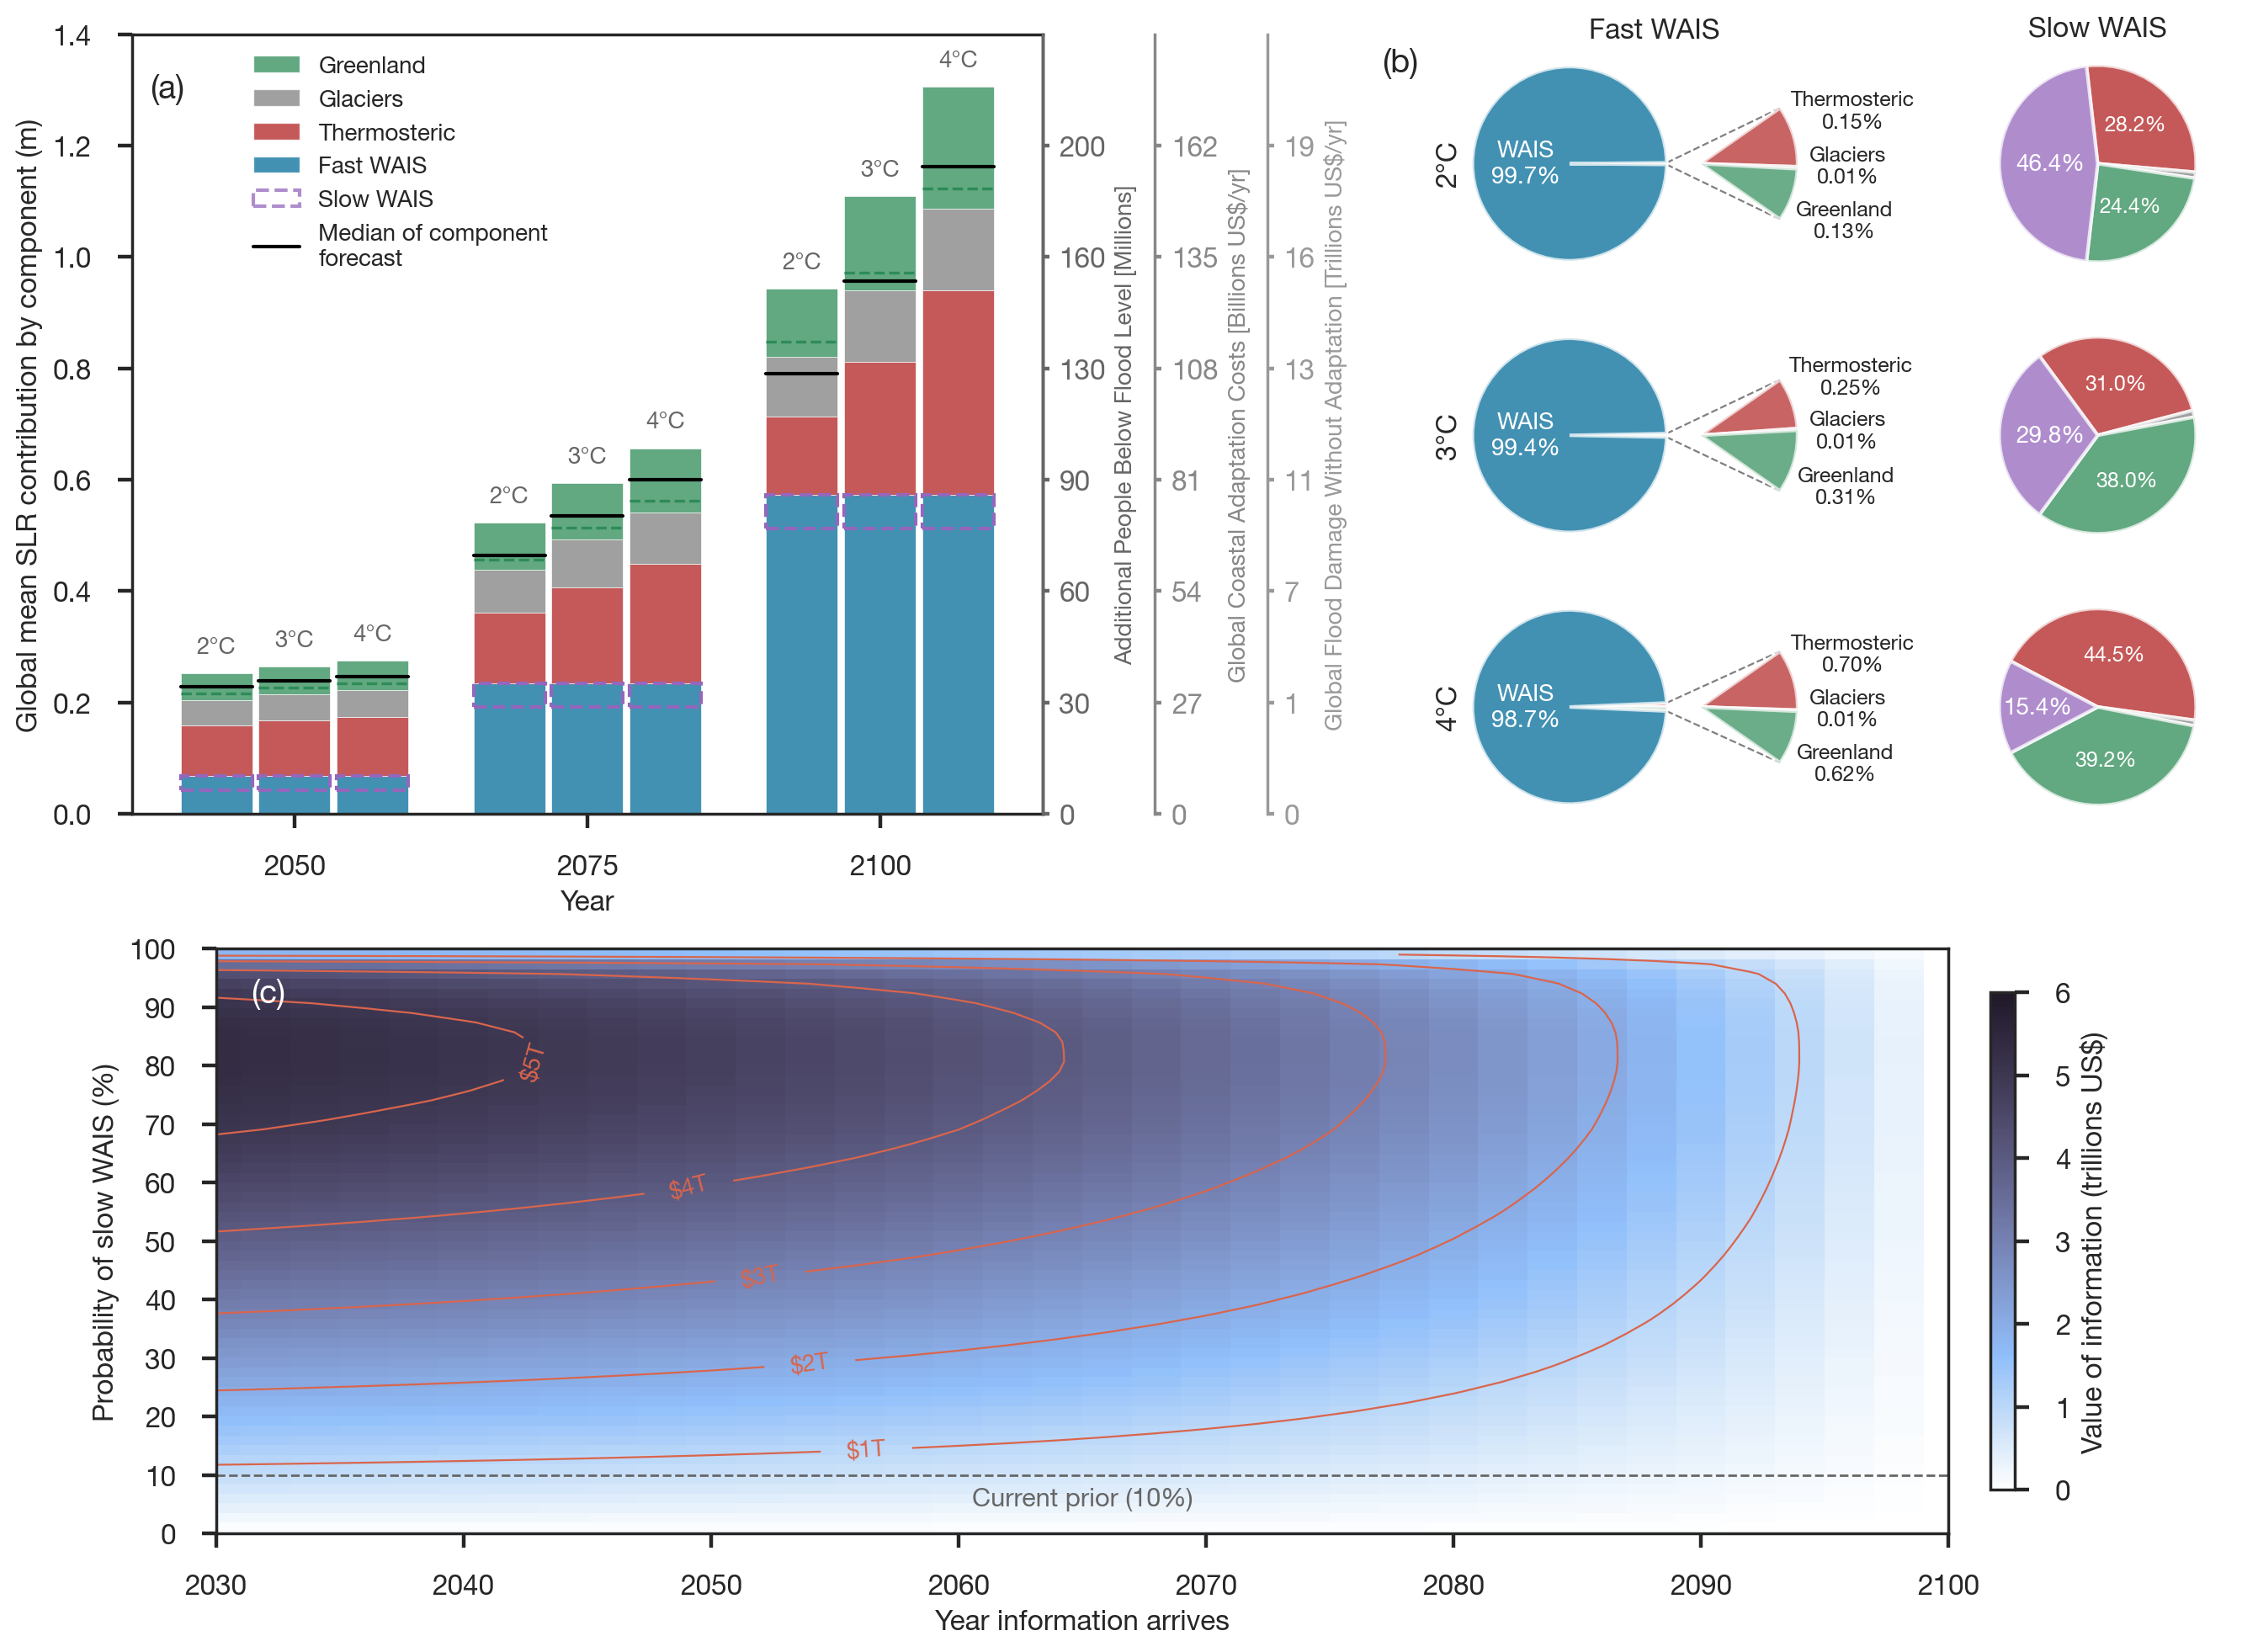
\includegraphics[width=\textwidth]{fig_slr_by_component_v2.png}
\caption{\textbf{Component contributions, variance decomposition, and value of information.}
\textbf{(a)} 21st century mean GMSLR contribution by component and respective societal costs. Green dashed lines within Greenland bars partition discharge anomaly (below) from SMB anomaly (above). The purple box shows how much WAIS will contribute if it loses mass slowly while the rest of the blue bar shows the potential SLR from rapid ice loss. 
\textbf{(b)} Variance-fractions at 2100. WAIS accounts for 97--99\% of total forecast variance when rapid ice loss is possible. Fan breakouts show the non-WAIS contributions. If WAIS loses mass slowly, the variance distributions fundamentally shift (right column) 
\textbf{(c)} Financial value of resolving WAIS uncertainty as a function of when information arrives. Contours and colormap in trillions US\$ based on coastal adaptation costs (Supplemental Material). The plot shows that information has more value if it arrives early enough to inform key decisions and if it provides sufficient confidence that WAIS will lose mass slowly, allowing planning around lower future sea levels.}
\label{fig:components_voi}
\end{figure}

The risks and costs to coastal communities helps to highlight the dichotomy between the two possible scenarios of fast vs slow WAIS mass loss, or equivalently, emissions-insensitive vs emissions sensitive (Figs. \ref{fig:ridge_projections} and \ref{fig:components_voi}a). The difference at the 5\% exceedance probability, one possible design threshold for coastal adaptation that we denote by stars in Fig. \ref{fig:ridge_projections}b, is 1.4 m of sea-level rise by 2100 under the current policy warming trajectory (3 $^\circ$C). This difference translates into roughly 260M more people exposed to annual flood risks, US\$182B/yr in coastal adaptation, and US\$18.2T/yr ($\sim$16\% global GDP per year) in coastal flood damages without further adaptation. These large numbers reflect global population densities, with the highest densities near coastlines, and the fact that the locations of coastal communities and infrastructure are calibrated to lower sea levels. For intuition, the fast-WAIS scenario at 5\% exceedance implies an order of magnitude more sea level rise in the next 75 years than was experienced in the past 125 years, while the slow-WAIS scenario implies a factor of 3.5 more rise.

Resolving the question of WAIS mass loss rates is among the most financially consequential goals in modern science (Fig.~\ref{fig:components_voi}c). A value-of-information analysis shows that perfect knowledge of whether WAIS will lose mass slowly or rapidly is worth of order US\$5T in avoided costs, with the value peaking when confidence in a slow-WAIS future reaches 80\% and the information arrives early enough to inform infrastructure decisions. The value decays with time because late-arriving information leaves fewer years of decisions to improve, and because all forecasts, including this study, degrade as they extend beyond their calibration bounds. These numbers frame the research investment question in concrete terms: even partial reduction of WAIS uncertainty, well short of perfect knowledge, would justify annual research expenditures orders of magnitude above current levels. The return on that investment is determined by how quickly the observations can narrow the range of WAIS outcomes, which depends on both the rate of data collection and the development of reliable process models, like those used in the IPCC, capable of providing explanatory insights that underscore deep understanding of ice sheets and climate. 

Our forecast identifies a single measurement that would do more to reduce sea-level uncertainty than any other: the rate of West Antarctic ice loss over the next two decades. If WAIS mass loss continues near current rates through the 2030s and 2040s, that would build the case for the slow-WAIS scenario and allow the forecast to narrow toward the predictable, lower, emissions-sensitive range where adaptation costs are more manageable. If instead grounding-line retreat accelerates beyond the pace of our central scenario, the distribution would shift toward higher outcomes and 1.5--2 m of rise would move from a tail risk to a planning baseline. Either outcome would reshape coastal adaptation worldwide and would justify investment well beyond current levels. The observations needed to distinguish these futures can be made within a generation, but only if the observing systems and research programs are sustained and expanded at a scale that reflects the costs at stake.

Scientific research is a necessary condition for providing actionable information for coastal adaptation, but it is as likely as not that further research will add to the growing evidence to support rapid WAIS mass loss rather than build confidence in a slow-WAIS future \citep{Fricker2025}. Sustaining a wide range of uncertainties that admit $<1$ m and $> 2$ m of GMSLR in 2100 at 10\% probabilities, will force decisions on coastal planning, adaptation, and managed retreat that impact millions of lives and cost billions of dollars to be made under large uncertainties. The extent of these uncertainties in terms of lives, property, and ecosystems raises the question: Can we take action to increase the potential stability of West Antarctica? How much harm to people and the environment can we prevent? Recently, some research directions have been proposed to answer this question \citep{MacAyeal2024} with initial models of glacier interventions aimed at stabilizing WAIS show promise \citep{Meyer2026}. As with any nascent research, there are many unresolved questions about the feasibility, unintended consequences, and governance of these interventions \citep{Siegert2025}. There are risks in intervening to remediate the West Antarctic Ice Sheet and slow its loss and the logistical challenges will undoubtedly be great, but these risks and challenges must be weighed against the risks and challenges of sea-level rise as described in this study. There is no zero risk, zero cost response to sea level rise. The costs and challenges are real and must be borne regardless of what decisions are made. The questions are how much cost, how much challenge, and how much harm. The answers hinge on how fast West Antarctica will lose ice, and nothing short of a virtual guarantee in slow WAIS mass loss provides comfort for the world's coastlines.   


%\subsection*{Broader implications}

%The data-driven framework presented here is not a replacement for process models, which remain essential for understanding the mechanisms of ice-sheet change. Our framework is complementary: an independent, data-driven estimate that makes its assumptions and limitations explicit, provides an observational benchmark against which process models can be tested, and produces conditional distributions that reflect what the data currently support. We consider robust, well-calibrated process models to be high-value targets for research and development, but the evidence suggests these models are not ready to be used for planning that costs billions of dollars and impacts millions of lives.

%We emphasize that the disconnect between the high costs of sea-level rise and the large uncertainties in current sea-level projections is a consequence of chronic under-investment compounded by the lack of institutional homes able to focus on translating knowledge gained through basic scientific research into forecasts for coastal communities in the way that, for example, the National Weather Service has traditionally done \citep{Catania2022}. A specific example is that modeling efforts for ISMIP6, which informed IPCC AR6 projections, were largely unfunded, leading to a dearth of model runs and near-absence of model parameter-sensitivity studies \citep{Aschwanden2021}. The world is going to endure high costs from sea-level rise (Fig. \ref{fig:ridge_projections}b). The questions are: how high will those costs be, and will we invest now to understand where and how to target funding to reduce the harm to people, ecosystems, and infrastructure, or continue on our current path? Our analysis shows that this investment must be directed along two independent axes---reducing emissions to compress the predictable components, and understanding and potentially stabilizing the West Antarctic Ice Sheet to address the dominant, emission-insensitive uncertainty that defines the upper bound of 21st-century sea-level rise.


%% ================================================================
%% REFERENCES
%% ================================================================

\bibliographystyle{agufull08}
\bibliography{references}

\end{document}     